%%
%% Author: Alexander Telich
%% 2/14/18
%%

% Preamble
\documentclass[11pt]{article}
\usepackage[utf8]{inputenc}
\usepackage{amsmath}

% Packages
\usepackage{a4wide}
\usepackage{listings}
\usepackage{indentfirst}
\usepackage{graphicx}

\lstdefinestyle{mystyle}{
basicstyle=\footnotesize,
breakatwhitespace=false,
breaklines=true,
captionpos=b,
keepspaces=true,
numbers=left,
numbersep=5pt,
showspaces=false,
showstringspaces=false,
showtabs=false,
tabsize=2
}

\lstset{style=mystyle}

\author{Alexander Telich}
\title{EECS 531 A1 Exercise 4}
\date{February 19, 2018}
\graphicspath{C:/Users/ateli/Documents/School/Spring 2018/EECS 531/Assignments/531_A1/A1/Exercise4}

% Document
\begin{document}
    \maketitle
    \section{ROC Curve Generation}\label{sec:exercise4}
    \subsection{Finding a way to classify FPR and TPR}\label{subsec:1.FPR and TPR}
    \setlength\parindent{24pt}
    The main issue that I had while completing this part was a way to generate the
    false positive rate and the true positive rate for my Harris Corner Detector.
    To do this I ran my corner detector and found a list of the detected corners.
    I then plotted this against the same set of corners to get the ROC curve.
    Aside from counting each one of the pixels, I could not determine a true positive rate.

    \section{Code}\label{sec:codeExplanation}
    \lstinputlisting[language=Python]{Exercise4.py}

    \begin{figure}[h]
        \caption{ROC Curve}
        \centering
        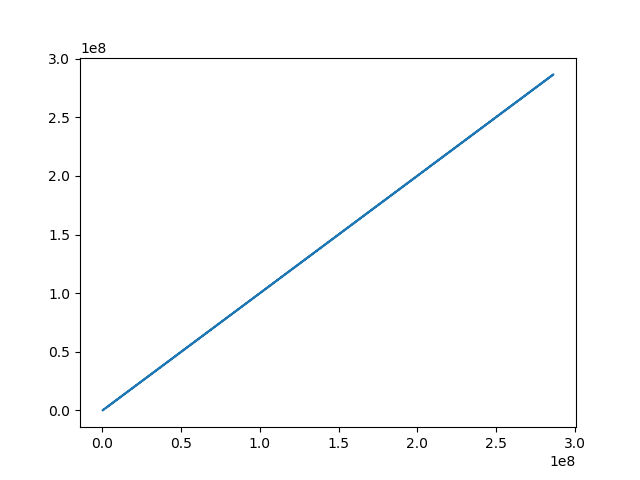
\includegraphics[scale=0.7]{myplot.png}
    \end{figure}



\end{document}
\begin{document}



\end{document}
\begin{document}



\end{document}